% !TeX root = ../paper.tex
\begin{figure}[!t]
\centering
\setlength{\parskip}{0pt}
\setlength{\abovecaptionskip}{\baselineskip}
\setlength{\belowcaptionskip}{0pt}
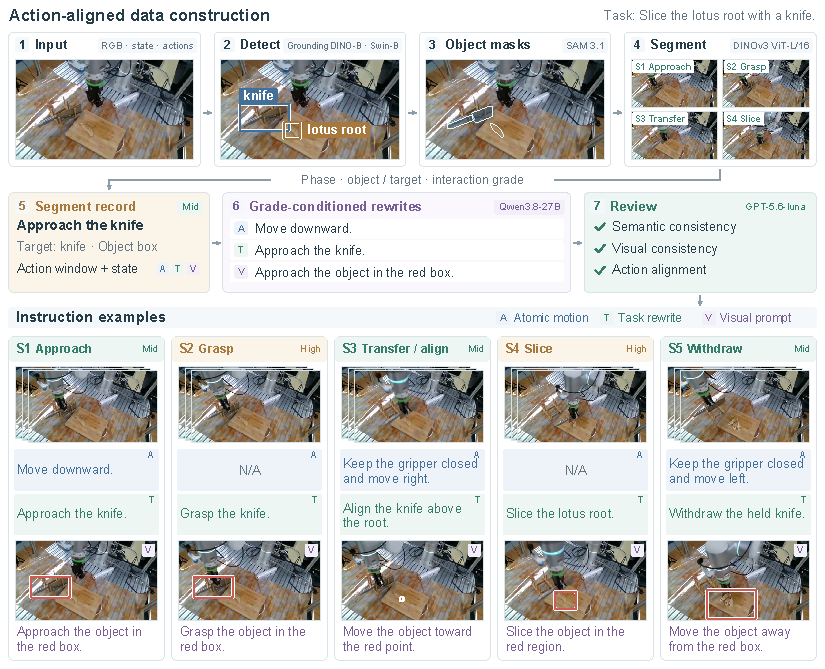
\includegraphics[width=\textwidth]{figures/appendix_action_aligned_pipeline_v12.pdf}\par\nointerlineskip
\caption{Action-aligned data construction illustrated with an RH20T
knife-and-lotus-root demonstration. Top: visual evidence extraction,
action-aligned segmentation, segment recording, grade-conditioned rewriting,
and consistency review. Bottom: atomic-motion (A), task-language (T), and
visual-prompt (V) examples for approach, grasp, transfer/alignment, slicing,
and withdrawal. N/A indicates that atomic-motion rewriting is excluded for
High-interaction segments.}
\label{fig:appendix-action-aligned-pipeline}
\end{figure}
